\section{Равномерное приближение заданной функции полиномами}

\begin{theorem}[О приближении по $\Delta$-последовательности]
    Пусть функции $D_n(x)$ удовлетворяют условиям:

    \begin{enumerate}
        \item $D_n(x)$ интегрируема на $[-\omega; \omega] \; (\omega > 0)$
        \item $D_n(-x) = D_n(x)$
        \item $D_n(x) \geq 0$
        \item $\ds\int_{-\omega}^\omega D_n(x) dx = 1$
        \item 
            $\{ D_n(x) \}$ равномерно сходится к $0$ на 
            $[-\omega; -\delta] \cup [\delta; \omega] \quad
            \forall \delta \geq 0 \quad \delta < \omega$

            Если $f(x)$ непрерывна на $[a - \omega; b + \omega]$, то
            $\{ f_n(x) \} : f_n(x) = 
            \ds\int_{-\omega}^\omega f(x + t) D_n(t) dt$ сходится равномерно 
            на $[a; b]$ к $f(x)$
    \end{enumerate}
\end{theorem}
\begin{proof}
    $f(x)$ непрерывна на $[a - \omega; b + \omega] \implies f(x)$ ограничена
    и равномерно непрерывна на $[a - \omega; b + \omega]$, то есть
    $\forall x \in [a - \omega; b + \omega] \quad |f(x)| \leq C$ и
    $\forall \varepsilon > 0 \quad \exists \delta_\varepsilon > 0 \quad
    \forall |t| \leq \delta_\varepsilon < \omega$ имеет место
    $|f(x + t) - f(x)| < \frac{\varepsilon}{2}$ при $x \in [a; b]$

    \begin{align*}
        |f_n(x) - f(x)| &= 
        \abs{\ds\int_{-\omega}^\omega f(x + t) D_n(t) dt - f(x) \cdot \ds\int_{-\omega}^\omega D_n(t) dt}
        = \abs{\ds\int_{-\omega}^\omega (f(x+t) - f(x)) D_n(t) dt} = \\ 
        &= \abs{\ds\int_{|t| \leq \delta} (f(x+t) - f(x)) D_n(t) dt + \ds\int_{\delta \leq |t| \leq \omega} (f(x+t) - f(x)) D_n(t) dt} \leq \\
        &\leq \ds\int_{|t| \leq \delta} |(f(x+t) - f(x)) D_n(t) dt| + \ds\int_{\delta \leq |t| \leq \omega} (|f(x+t)| + |f(x)|) D_n(t) dt < \\
        &< \frac{\varepsilon}{2} \ds\int_{|t| < \delta} D_n(t) dt + 4C \sup_{\delta \leq |t| \leq \omega} D_n(t) \cdot (\omega - \delta) <
        \frac{\varepsilon}{2} + 4C \cdot \sup_{\delta \leq |t| \leq \omega} D_n(t) \cdot (\omega - \delta)
    \end{align*}

    Так как $\{ D_n(t) \}$ равномерно сходится к $0$ на $[-\omega; -\delta] \cup
    [\delta; \omega] \implies$ для нашего $\varepsilon$ $\exists N_\varepsilon
    \quad \forall n \geq N_\varepsilon \quad 
    4C \cdot \ds\sup_{\delta \leq |t| \leq \omega} D_n(t) (\omega - \delta) < 
    \frac{\varepsilon}{2} \implies
    \forall \varepsilon > 0 \quad \exists N_\varepsilon \quad \forall n \geq N_\varepsilon
    \forall x \in [a; b] \quad |f_n(x) - f(x)| < \varepsilon \bydef \{ f_n(x) \}$
    равномерно сходится к $f(x)$ на $[a; b]$.
\end{proof}

\begin{remark}

\end{remark}


\begin{theorem}[Первая Теорема Вейерштрасса о равномерном приближении 
непрерывной функции алгебраическими полиномами]
    Если $f(x)$ непрерывна на $[a; b]$, то существует последовательность
    алгебраических полиномов, равномерно сходящаяся на $[a; b]$ 
    к функции $f(x)$.
\end{theorem}
\begin{proof}
    Рассмотрим $D_n(x) = C_n \left( 1 - \frac{x^2}{\omega^2} \right)^n$ с
    дополнительным условием:
    \[ \ds\int_{-\omega}^\omega D_n(t) dt = 1,\, \text{то есть } \,
    C_n = \frac{1}{\ds\int_{-\omega}^\omega \left(1 - \frac{x^2}{\omega^2}\right)^n dx} \]
    
    Докажем, что $D_n(x)$ образует $\Delta$-образную последовательность.

    \begin{enumerate}
        \item $D_n(x) \geq 0 \quad x \in [-\omega; \omega]$
        \item $D_n(-x) = D_n(x)$
        \item $D_n(x)$ интегрируема на $[-\omega; \omega]$
    \end{enumerate}

    Оценим $C_n$ при $n \geq 1$:

    \begin{align*}
        \ds\int_{-\omega}^\omega \left( 1 - \frac{x^2}{\omega^2} \right)^n dx \geq
        \ds\int_{-\omega / \sqrt{n}}^{\omega / \sqrt{n}} \left( 1 - \frac{x^2}{\omega^2} \right)^n dx \geq
        \ds\int_{-\omega / \sqrt{n}}^{\omega / \sqrt{n}} \left( 1 - n\frac{x^2}{\omega^2} \right) dx = \\
        = \left( x - \frac{n x^3}{3 \omega^2} \right) \Bigg|_{-\omega / \sqrt{n}}^{\omega / \sqrt{n}} =
        2 \left(\frac{\omega}{\sqrt{n}} - \frac{n \omega^3}{n \sqrt{n} \cdot 3 \omega^2}\right) =
        \frac{4}{3} \frac{\omega}{\sqrt{n}} \implies C_n \leq \frac{3 \sqrt{n}}{4 \omega}
    \end{align*}

    \[ D_n(x) = C_n \left(1 - \frac{x^2}{\omega^2}\right)^n \leq 
    \frac{3 \sqrt{n}}{4\omega} \left(1 - \frac{\delta^2}{\omega^2}\right)^n \]

    то есть \[ 0 \leq D_n(x) \leq \frac{3}{4 \omega} 
    \frac{n^{1/2}}{ \left(\frac{1}{1 - \delta^2 / \omega^2}\right)^n } \quad
    \left( \frac{n^k}{a^n} \approach{n \to \infty} 0 \right)\]

    $\implies \{ D_n(t) \}$ равномерно сходится к $0$ на $[-\omega; -\delta] \cup
    [\delta; \omega] \implies \{ D_n(x) \}$ --- $\Delta$-образная последовательность.

    Тогда по Теореме о равномерном приближении $\Delta$-образной последовательности
    $f_n(x) = \ds\int_{-\omega}^\omega f(x + t) D_n(t) dt$ равномерно сходится
    на $[a; b]$ к $f(x)$ если $f(x)$ будет непрерывной на $[a - \omega; b + \omega]$.

    Рассмотрим $f^*(x) = \begin{cases}
        0, \quad &x \not\in [a; b] \\
        f(x), \quad &x \in [a; b]
    \end{cases}$

    Сначала будем считать, что $f(a) = f(b) = 0$. Тогда $f^*(x)$ непрерывна на
    отрезке $[a - \omega; b + \omega]$ и последовательность $\{ f_n(x) \} : 
    f_n(x) = \ds\int_{-\omega}^\omega f^*(x + t) D_n(t) dt$ равномерно сходится
    на $[a; b]$ к $f^*(x) = f(x)$, при этом $D_n(x)$ и $f_n(x)$ --- 
    алгебраические полиномы степени $2n$.

    От дополнительного условия $f(a) = f(b) = 0$ можно избавиться рассмотрев
    вместо функции $f(x)$ функцию 
    \[ g(x) = f(x) - f(a) - \frac{x - a}{\omega} (f(a + \omega) - f(a)) \]

    которая удовлетворяет условию $g(a) = g(a + \omega) = 0$ и отличается от
    $f(x)$ на слагаемое, которое является алгебраическим полиномом 
    первой степени.
\end{proof}


\begin{theorem}[Вторая Теорема Вейерштрасса о равномерном приближении
непрерывной периодической функции последовательностью полиномов]
    Если $f(x)$ непрерывна и периодична, то существует последовательность
    тригонометрических полиномов с тем же периодом, равномерно сходящаяся
    к $f(x)$.
\end{theorem}
\begin{proof}
    Рассмотрим $D_n(x) = C_n(\cos \frac{\pi x}{2 \omega})^{2n}$ с дополнительным
    условием $\ds\int_{-\omega}^\omega D_n(x) dx = 1$

    \[ \left(C_n = \frac{1}{\ds\int_{-\omega}^\omega \left(\cos \frac{\pi x}{2 \omega}\right)^{2n} dx}\right) \]

    \begin{enumerate}
        \item $D_n(-x) = D_n(x)$
        \item $D_n(x) \geq 0$
    \end{enumerate}

    Оценим $C_n$:

    \begin{align*}
        &\left(\cos \frac{\pi x}{2 \omega}\right)^{2n} = 
        \left(1 - \sin^2 \frac{\pi x}{2 \omega}\right)^n \geq
        1 - n \sin^2 \frac{\pi x}{2 \omega} \;
        \over{|\sin x| \leq |x| \leq \frac{\pi}{2}}{\geq} \;
        1 - n \left(\frac{\pi x}{2 \omega}\right)^2 \\
        &\implies \ds\int_{-\omega}^\omega \left(\cos \frac{\pi x}{2 \omega}\right)^{2n} dx >
        \ds\int_{-\frac{2 \omega}{\pi \sqrt{n}}}^{\frac{2 \omega}{\pi \sqrt{n}}} \left(\cos \frac{\pi x}{2 \omega}\right)^{2n} \geq
        \ds\int_{-\frac{2 \omega}{\pi \sqrt{n}}}^{\frac{2 \omega}{\pi \sqrt{n}}} \left( 1 - n \frac{\pi^2 x^2}{4 \omega^2} \right) dx = \\
        &= \left( x - \frac{n \pi^2 x^3}{12 \omega^2} \right) \Bigg|_{-\frac{2 \omega}{\pi \sqrt{n}}}^{\frac{2 \omega}{\pi \sqrt{n}}} =
        2 \left( \frac{2 \omega}{\pi \sqrt{n}} - \frac{n \pi^2 8 \omega^3}{\pi^3 n \sqrt{n} 12 \omega^2} \right) =
        2 \left( \frac{2 \omega}{\pi \sqrt{n}} - \frac{2 \omega}{3 \pi \sqrt{n}} \right) = \\
        &= 2 \cdot 2 \cdot \frac{2}{3} \cdot \frac{\omega}{\pi \sqrt{n}} = \frac{8 \omega}{3 \pi \sqrt{n}}
        \implies C_n \leq \frac{3 \pi \sqrt{n}}{8 \omega} 
        \over{\delta \leq |x| \leq \omega}{\implies} 0 \leq D_n(x) \leq \frac{3 \pi \sqrt{n}}{8 \omega} \left(1 - \sin^2 \frac{\pi \delta}{2 \omega}\right)^n
    \end{align*}

    $\forall x \in [-\omega; -\delta] \cup [\delta; \omega] \; n \approach{} 
    \infty \implies \{ D_n(x) \}$ равномерно сходится к $0$ на 
    $[-\omega; -\delta] \cup [\delta; \omega] \implies D_n(x)$ является
    $\Delta$-образной последовательностью.

    Так как $f(x)$ непрерывная периодическая функция с периодом $T$, то
    возьмём $2\omega = T,\, x \in [-\omega; \omega]$. Тогда по Теореме о
    равномерном приближении по $\Delta$-образной последовательности имеем:

    \begin{align*}
        f_n(x) &= \ds\int_{-\omega}^\omega f(x + t) D_n(t) dt \over{x + t = S}{=}
        \ds\int_{-\omega + x}^{\omega + x} f(S) D_n(S - x) dS = \\
        &= \ds\int_{-\omega + x}^{-\omega} f(S) D_n(S - x) dS +
        \ds\int_{-\omega}^\omega f(S) D_n(S - x) dS +
        \ds\int_{\omega}^{\omega + x} f(S) D_n(S - x) ds = \\
        &= \left/\begin{array}{lr}
            f(S) = f(S - 2 \omega)\\
            D_n(t - 2\omega) = D_n(S)
        \end{array}\right/ = 
        \ds\int_{-\omega + x}^{-\omega} f(S + 2\omega) D_n(S - x + 2\omega) ds + \\
        &+ \ds\int_{-\omega}^{\omega} f(S) D_n(S - x) ds +
        \ds\int_{\omega}^{\omega + x} f(S) D_n(S - x) ds = 
        \left/\text{в 1-м  } S + 2\omega = y\right/ = \\
        &= \ds\int_{\omega + x}^\omega f(y) D_n(y - x) dy +
        \ds\int_{-\omega}^{\omega} f(S) D_n(S - x) dS +
        \ds\int_{\omega}^{\omega + x} f(S) D_n(S - x) dS = \\
        &= \ds\int_{-\omega}^{\omega} f(S) D_n(S - x) dS
    \end{align*}

    По Теореме о приближении по $\Delta$-образной последовательности
    $f_n(x) = \ds\int_{-\omega}^{\omega} f(S) D_n(S - x) dS$ равномерно 
    сходится на $x \in [-\omega; \omega]$ к $f(x)$. Так как $f_n(x)$ и $f(x)$
    периодичны с $T = 2\omega$, то равномерная сходимость имеет место при
    любых $x$.
\end{proof}

\begin{remark}
    Можно показать, что $f_n(x) = \ds\sum_{k = 0}^n \left( a_k \cdot \cos
    \frac{\pi k x}{\omega} + b_k \cdot \sin \frac{\pi k x}{\omega} \right)$
\end{remark}


\begin{definition}
    Выражение $T_n(x) = \ds\sum_{k = 0}^n \left( a_k \cos kx + b_k \sin kx \right)$
    называют тригонометрическим полиномом.
\end{definition}

\begin{definition}
    Говорят, что последовательность $\{ f_n(x) \}$ сходится к функции $f(x)$
    в среднем на $[a; b]$, если $\dslimn \ds\int_a^b (f_n(x) - f(x))^2 dx = 0$
\end{definition}


\begin{theorem}[О связи равномерной сходимости и сходимости в среднем]
    Если $\{ f_n(x) \}$ сходится равномерно к $f(x)$ на $[a; b] \implies
    \{ f_n(x) \}$ сходится в среднем к $f(x)$ на $[a; b]$.
\end{theorem}
\begin{proof}
    $\{ f_n(x) \}$ равномерно сходится к $f(x)$ на $[a; b] \implies
    \forall \varepsilon > 0 \quad \exists N_\varepsilon \quad \forall n \geq
    N_\varepsilon \quad \forall x \in [a; b] \quad |f_n(x) - f(x)| < \varepsilon
    \implies \ds\int_a^b [f_n(x) - f(x)]^2 dx < \varepsilon^2 (b - a) \dn \varepsilon^*
    \implies$ получили определение $\dslimn \ds\int_a^b (f_n(x) - f(x))^2 dx = 0 
    \implies \{ f_n(x) \}$ сходится в среднем на $[a; b]$ к $f(x)$.
\end{proof}


\begin{theorem}[О сходимости $\ds\int_a^b f_n(x) g(x) dx$]
    Пусть $f_n(x)$ интегрируется на $[a; b]$. $\{ f_n(x) \}$ сходится в среднем
    на $[a; b]$ к $f(x)$, интегрируемой на $[a; b]$. $g(x)$ --- интегрируема
    на $[a; b]$.

    Тогда $\ds\limn \ds\int_a^b f_n(x) g(x) dx = \ds\int_a^b f(x) g(x) dx$.
\end{theorem}
\begin{proof}
    Используем неравенство Коши-Буняковского для интервалов:
    \[
        \abs{\ds\int_a^b \varphi(x) \cdot \psi(x) dx} \leq 
        \sqrt{ \ds\int_a^b \varphi^2 (x) dx \ds\int_a^b \psi^2(x) dx }
    \]

    \[
        0 \leq \abs{\ds\int_a^b f_n(x) g(x) dx - \ds\int_a^b f(x) g(x) dx} =
        \abs{\ds\int_a^b (f_n(x) - f(x)) g(x) dx} \leq
        \sqrt{ \ds\int_a^b (f_n(x) - f(x))^2 dx \ds\int_a^b g(x)^2 dx }
    \]
    (левое и правое выражения неравенства $\approach{} 0 \implies$ среднее
    выражение $\approach{} 0$)
\end{proof}


\begin{theorem}[О приближении в среднем интегрируемой функции непрерывной]
    Пусть $f(x)$ интегрируема на $[a; b]$. Тогда $\forall \varepsilon > 0 \quad
    \exists f_\varepsilon(x)$ --- непрерывная на $[a; b]$ и принимающая 
    заданные значения в точках $x = a$ и $x = b$:
    \[ \ds\int_a^b [f(x) - f_\varepsilon(x)]^2 dx < \varepsilon \]
\end{theorem}
\begin{proof}
    Пусть $R$ --- произвольное разбиение отрезка $[a; b]: \:
    a = x_0 < x_1 < x_2 < \dots < x_n = b$

    $\Delta x_i = x_{i + 1} - x_i, \, \Delta = \ds\max_{0 \leq i \leq n - 1}
    \Delta x_i$ --- диаметр $R$.

    Так как $f(x)$ интегрируема на $[a; b] \implies f(x)$ --- ограничена на
    $[a; b]: \: \exists M > 0 \quad \forall x \in [a; b] \quad |f(x)| \leq M$
    и выполняется критерий интегрируемости 
    \[ \ds\lim_{\Delta \to 0} \ds\sum_{i = 0}^{n - 1} \omega_i \Delta x_i = 0 \]

    $\omega_i = \ds\sup_{x', x'' \in [x_i; x_{i + 1}]} |f(x') - f(x'')|$ ---
    колебания $f(x)$ на $[x_i; x_{i + 1}]$.

    \begin{figure}[H]
        \centering
        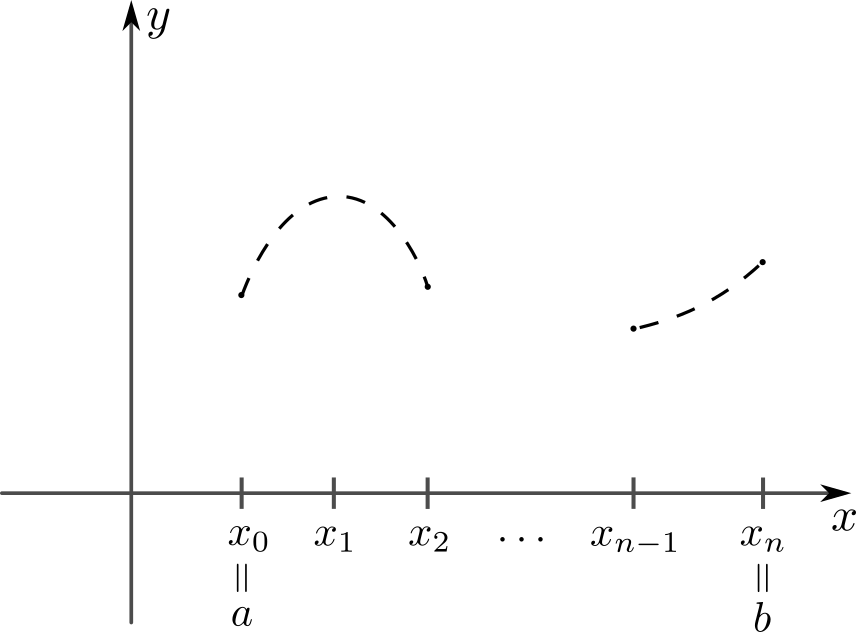
\includegraphics[width=0.5\textwidth]{images/approx_mean.png}
    \end{figure}

    Построим $f_\varepsilon(x)$ следующим образом: $f_\varepsilon(x_i) = f(x_i)
    \quad \forall i = \overline{1, n - 1}$ на отрезке $[x_i; x_{i + 1}]$ ---
    линейная функция, а при $x = a, \, x = b$ функция $f_\varepsilon(x)$
    принимает заданные значения.

    Очевидно, что построенная $f_\varepsilon(x)$ --- непрерывна и
    $\forall x \in [x_i; x_{i + 1}] \quad i = \overline{1, n - 2}$ выполняется
    \begin{align*}
        &\min [f(x_i); f(x_{i + 1})] \leq 
        f_\varepsilon(x) \leq \max [f(x_i); f(x_{i + 1})] \\
        &\implies \begin{cases}
            f(x) - f_\varepsilon(x) \leq f(x) - \min [f(x_i); f(x_{i + 1})] \leq \omega_i \\
            f_\varepsilon(x) - f(x) \leq \max [f(x_i); f(x_{i + 1})] - f(x) \leq \omega_i
        \end{cases} \\
        &\implies |f(x) - f_\varepsilon(x)| \leq \omega_i
    \end{align*} 

    \begin{align*}
        [f(x) - f_\varepsilon(x)]^2 &= |f(x) - f_\varepsilon(x)|^2 = \\
        &= |f(x) - f_\varepsilon(x)| \cdot |f(x) - f_\varepsilon(x)| \leq \\ 
        &\leq (|f(x)| + |f_\varepsilon(x)|) \cdot \omega_i \leq 2 M \cdot \omega_i
    \end{align*}

    При $x \in [x_0; x_1]$ (то есть $[a; x_1]$) и 
    $x \in [x_{n - 1}; x_n]$ (то есть $[x_{n - 1}; b]$):

    \[ [f(x) - f_\varepsilon(x)]^2 \leq [|f(x)| + |f_\varepsilon(x)|]^2 \leq (M + M_1)^2 \]
    где $M_1 = \max \{ M; |f_\varepsilon(a)|; |f_\varepsilon(b)| \}$

    Тогда $\ds\int_a^b (f(x) - f_\varepsilon(x))^2 dx = 
    \ds\sum_{i = 0}^{n - 1} \ds\int_{x_i}^{x_i + 1} [f(x) - f_\varepsilon(x)]^2 dx \leq
    2M \ds\sum_{i = 1}^{n - 2} \omega_i \Delta x_i + 2(M + M_1)^2 \cdot \Delta$

    Таким образом правая часть $\approach{} 0$ при $\Delta \approach{} 0$,
    значит $\forall \varepsilon > 0 \quad \exists R$ --- разбиение отрезка
    $[a; b] \implies \exists f_\varepsilon(x)$ --- непрерывна на $[a; b]$ с
    заданными значениями на концах:
    \[ \ds\int_a^b [f(x) - f_\varepsilon(x)]^2 dx < \varepsilon \]
\end{proof}

\begin{corollary}
    Если $f(x)$ интегрируема на отрезке $[a; b]$, то $\forall \varepsilon > 0
    \quad \exists f_\varepsilon(x)$ --- непрерывная на $[a; b]$ и принимающая
    в точках $a$ и $b$ заданные значения:
    \[ \ds\int_a^b |f(x) - f_\varepsilon(x)|^2 dx < \varepsilon \]
\end{corollary}
\begin{proof}
    Получаем из предыдущей Теоремы с помощью неравенства Коши-Буняковского.
\end{proof}
